%% This is an example first chapter.  You should put chapter/appendix that you
%% write into a separate file, and add a line \include{yourfilename} to
%% main.tex, where `yourfilename.tex' is the name of the chapter/appendix file.
%% You can process specific files by typing their names in at the 
%% \files=
%% prompt when you run the file main.tex through LaTeX.
%% prompt when you run the file main.tex through LaTeX.
\chapter{Predicting Mercury Concentrations in the Atmosphere in Latin America using GEOS-Chem }
%% BACKGROUND
\section{Background}
\begin{flushleft}
Comparing models to observation data is essential to validate the predictions made by the models as well as offer insights on how to improve the models[cite]. Models and observation networks have a symbiotic relationship. For instance, observation networks have limited spatial and temporal coverage hence yet models can product information about the state of various locations at once. Consequently

Anthropogenic Hg sources, including ASGM, have been quantified in numerous prior studies using different methodologies. Bottom-up estimates leverage collected data on underlying activities and multiply activity levels by emission factors to estimate regional and global totals. For instance, Figure \ref{fig:World_Hg_em} shows the most recent estimated spatial distribution of anthropogenic Hg emissions as reported in the 2018 Global Mercury Assessment, which also estimated ASGM Hg emissions to be 838 tonnes with an uncertainty range of 675-1000 tonnes for 2015\cite{united_nations_environment_programme_technical_2019}. Moreover, Streets et al. (2019) tested six different proxies for scaling emissions to other years and used an average value to scale the inventory of emissions to the year 2015 thus estimating that ASGM was the largest source and responsible for 775 Mg of emissions\cite{streets_global_2019}. Furthermore, Muntean et al. (2014) found that poverty in  gold ore rich countries (as measured by the GINI index \cite{sadefo_kamdem_nice_2012}, where available) was correlated with data on ASGM production activity when they used a poverty-based approach to estimate that ASGM was responsible for 728.27 t of emissions in 2010 which was equivalent to 41.1\% of the global emissions\cite{muntean_evaluating_2018}. Such inventories are comprehensible, and their universal applicability enables worldwide coverage. However, the different assumptions on the activity data and emission factors induce significant uncertainty in the emission inventories. An additional bias in the bottom-up approach originates from the reliance on officially reported emissions data, which might cause differences in accuracy between countries and regions.
\begin{figure}[H]
  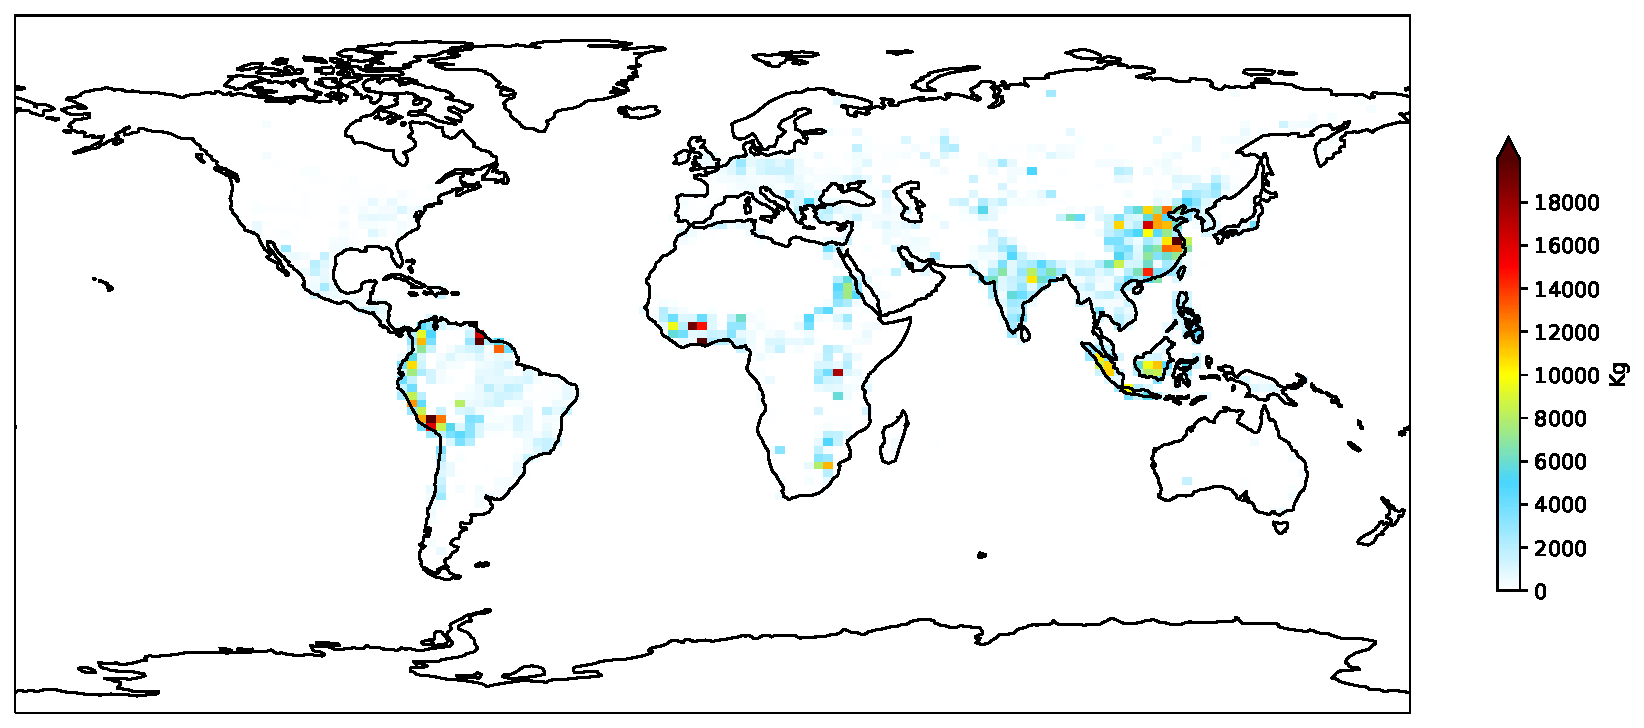
\includegraphics[width=0.8\textwidth]{templates/figures/06-12-22_total_Hg0-emissions-per-year_globally_001.pdf}
  \centering
  \caption{Spatial distribution of annual average Hg anthropogenic emissions for a 1 year period between July 2014 and July 2015}
  \label{fig:World_Hg_em}
\end{figure}
\FloatBarrier

National inventories are also a form of a bottom up inventory where countries identify and quantify the sources of mercury releases within their borders. Countries are required to include in their NAPs baseline estimates of the quantities of mercury used in ASGM and the produced estimate should have an accuracy of +/- 30\% and at worst +/- 50\% \cite{united_nations_environment_programme_estimating_2017}.
\end{flushleft}
\begin{flushleft}
On the contrary, top-down emission estimation approaches combine atmospheric transport and chemistry models with atmospheric concentration measurements to quantify emissions. Even though the atmospheric chemistry literature has various top-down method applications, no study explicitly constrains ASGM Hg emissions. For instance, Bousquet et al., 1999 applied top-down methods to infer surface fluxes of atmospheric CO\textsubscript{2} from observed concentrations\cite{bousquet_inverse_1999}. Furthermore, Kopacz et al., 2009, employed these techniques to quantify source contributions to ozone pollution at two adjacent sites on the U.S. west coast in the spring of 2006. Moreover, Stohl et al., 2010 determined the emissions of hydrochlorofluorocarbon and hydrofluorocarbon from four East Asian countries and the Taiwan region for the year 2008 using similar techniques. Hg emissions have also been constrained using top-down methods in Song et al., 2015 where they apply a top-down approach at a global scale to quantitatively estimate present-day Hg emission sources and critical parameters in GEOS-Chem to constrain the global biogeochemical cycle of Hg better. Moreover, Densler et al., 2017 used a top-down approach to quantify Hg emissions on a European scale based on the atmospheric Hg measurements conducted at the remote high altitude monitoring station, Jungfraujoch, Switzerland. 
\end{flushleft}
\begin{flushleft}
Herein we investigate the extent to which the GEOS-Chem model predicts the Hg concentrations in the atmosphere in regions with high ASGM activities such as the tropical regions of the world. Figure \ref{fig:World_Hg_em} leverages the most recent emission estimates of Hg emissions globally and it shows that regions such as South America, Africa, South East ASIA and China are the sources of the highest Hg anthropogenic emissions. The estimates from the GMA 18 further attribute the high Hg emission from South America and Africa to ASGM activities\cite{united_nations_environment_programme_technical_2019}. To our knowledge, there is a dearth of scientific studies investigating the extent to which models such as GEOS-Chem reproduce observed Hg concentrations in the atmosphere. The highly cited fact that that perpetuates the absence of such studies is the lack of monitoring data that researcher could use in modelling studies. However, the GMOS network has about 5 monitoring stations in Latin America whose data can be compared to modelling results. Moreover, the Wania Grouped deployed numerous passive air samplers (PAS)  in different locations across Latin America to monitor Hg concentration in the atmosphere thus providing data that can be compared to model outputs.Therefore, we compare the modelled Hg concentrations in the atmosphere to observed concentrations assess the GEOS-Chem models strengths and short comings in reproducing the observed Hg concentrations in the atmosphere. 
\end{flushleft}

%%----------------------------METHODS-------------------------------------------
\section{Methods}

\subsection{Case Study Region}
\begin{figure}[H]
  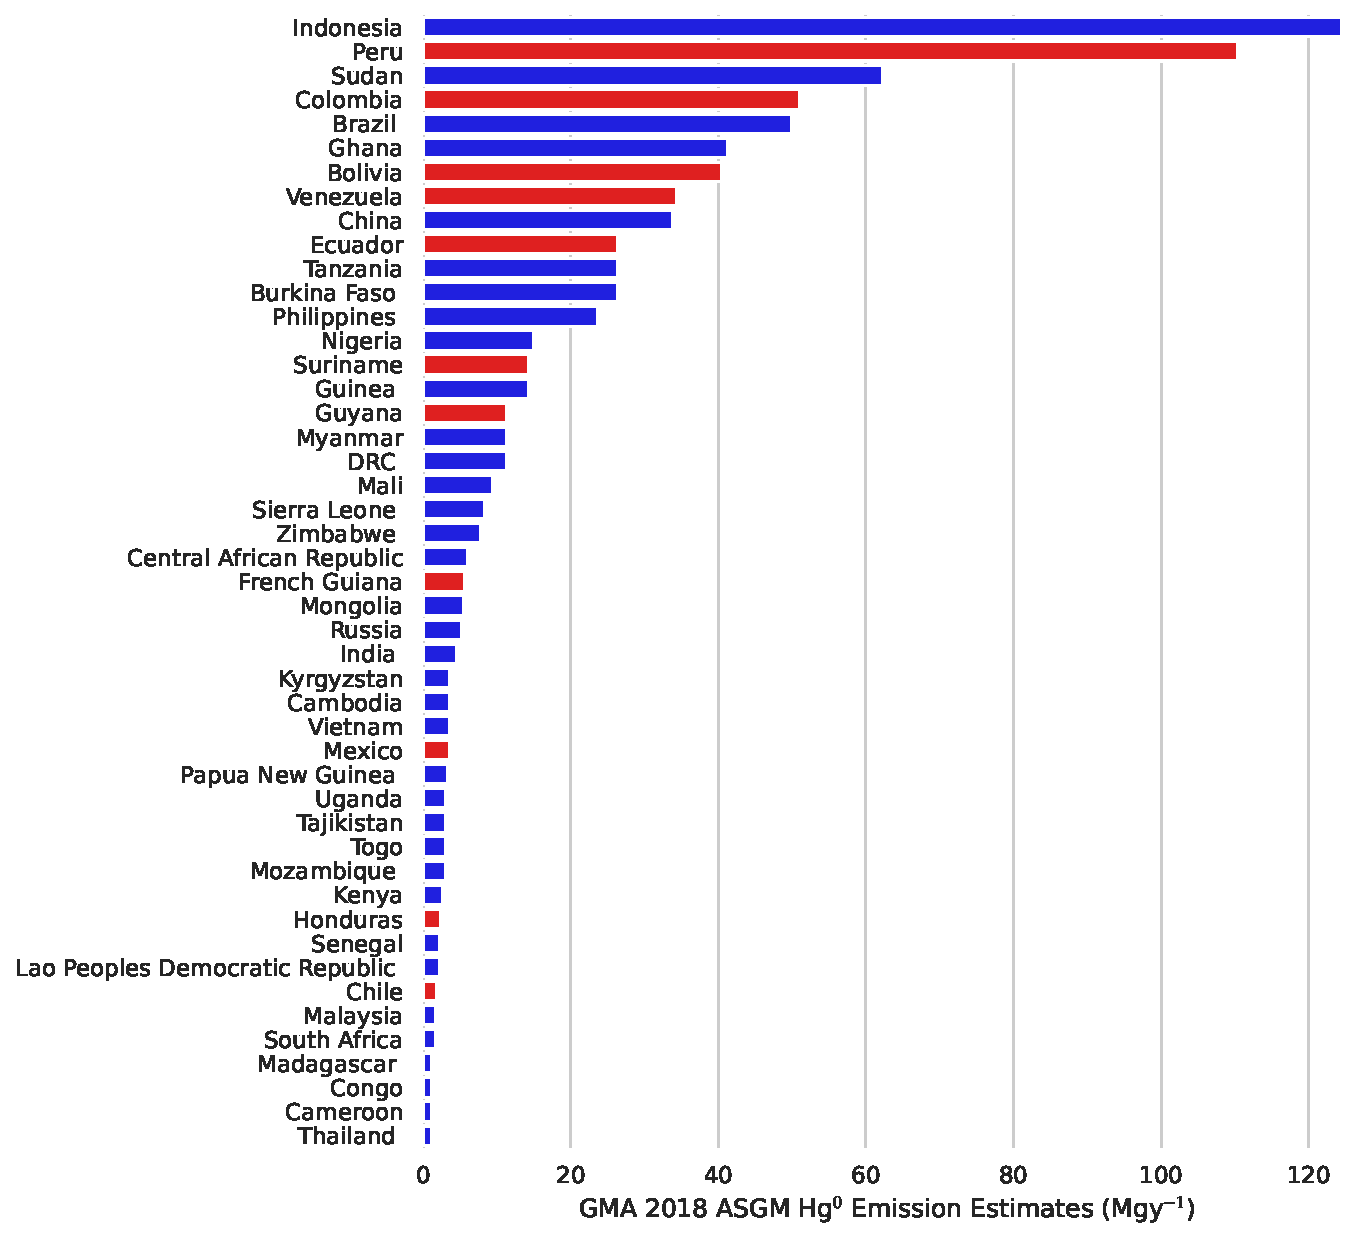
\includegraphics[width=0.8\textwidth]{templates/figures/07-14-22_gma2018_top-asgm-emmiting-countries.pdf}
  \centering
  \caption{Map showing the spatial distribution of the average Hg anthropogenic emissions in South America}
  \label{fig:Latam_Hg_em}
\end{figure}
\FloatBarrier
\begin{flushleft}
As reported by the GMA 2018, Peru is one of the top emitters of ASGM Hg. Additionally, the Madre de Dios region was estimated to have released the largest quantities of Hg to the environment and the atmosphere[AGC]. This rainforest region lies between Bolivia and Brazil and covers roughly 85,000 square kilometers. The region's name is derived from the name of a major river that runs through it, and smaller streams and rivers cross through it to provide transportation and fishing for indigenous communities. In addition, these waterways are the main sites of ASGM and, subsequently, Hg contamination. 
\end{flushleft}

\begin{flushleft}
Although Brazil nut, coffee, papaya, and cacao are cultivated, the land is primarily dominated by ASGM (Diringer et al., 2015, Caballero Espejo et al., 2018). (Diringer et al., 2015) estimate that ASGM land has increased by 400\% since 1999. As a result, 100,000 hectares of forest have been deforested, with 10\% occurring only in 2017 (Caballero Espejo et al., 2018). Researchers have found it difficult to verify the amount of hg imported and gold extracted from Madre de Dios (Cortés-McPherson, 2019, Swenson et al., 2011, Veiga et al., 2006) and the number of illegal miners, which Mr. Brack-Egg estimated in 2010 at 30,000 (Diringer et al., 2015, MINAM 2011, Swenson et al., 2011). It is estimated that around 180 tons of Hg enter the environment of Madre de Dios every year (MongoBay Latam, 2018, Servindi, 2018). However, these numbers are not very accurate and are, in part, contradictory. 
\end{flushleft}


\begin{flushleft}
Hg has been extensively studied in Madre de Dios, both in people and in the environment. Prior environmental measurements performed in Madre de Dios regarding the amount of Hg entering soil, air, and waterways reflected drastically different results between government estimates and international researchers. This demonstrates a need to generate further system-wide constraints on ASGM Hg use and pollution. Some studies focus on human health in the region (Gibb \& O'Leary, 2014), and others have bridged natural science perspectives with community engagement and trans-disciplinary approaches (Landon et al., 2015). Through leveraging national and global emission inventories, long-range measurements of Hg concentration in the atmosphere, and the GEOS-Chem Chemical Transport Model, this project complements previous studies and distinguishes itself from previous studies in this highly-studied region. Results will be generated for the Madre de Dios region and its surrounding areas that have high ASGM activity. 
\end{flushleft}
\begin{figure}[H]
  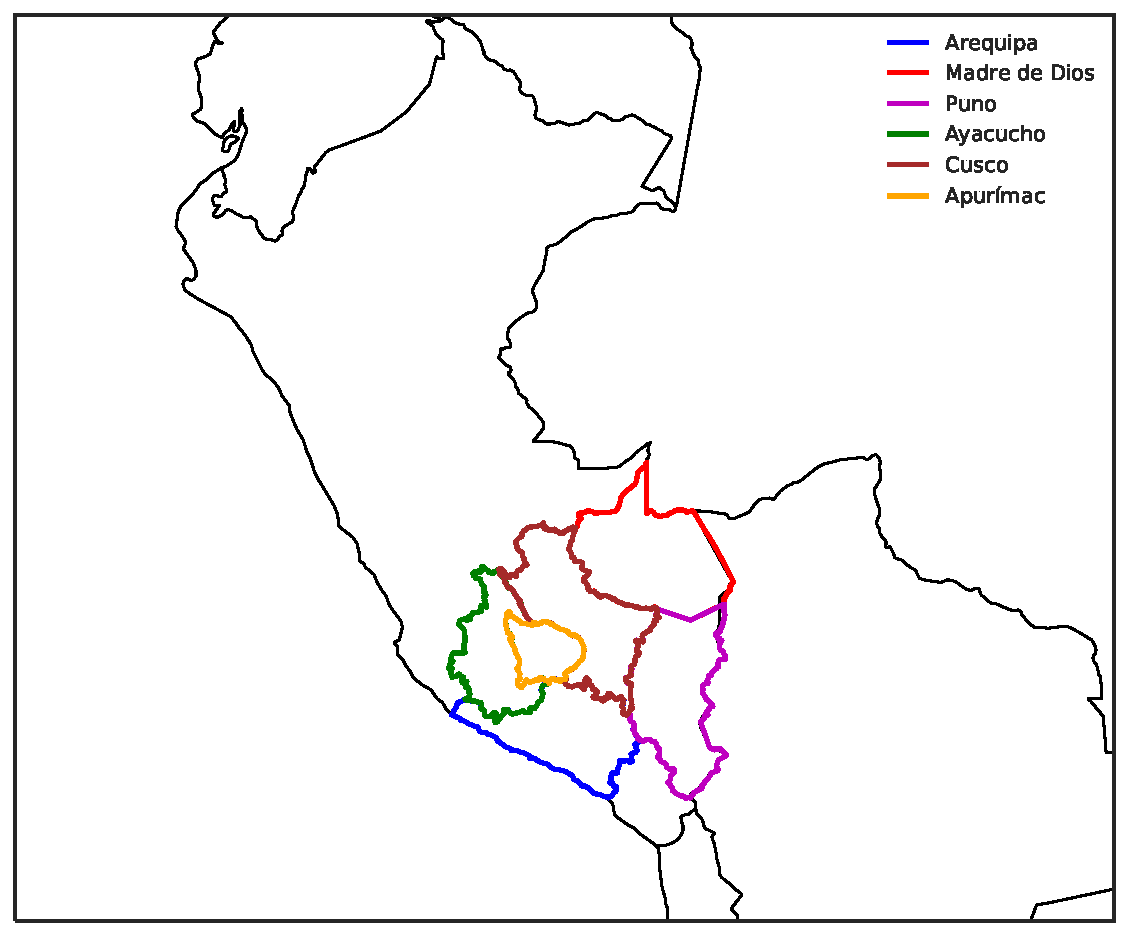
\includegraphics[width=0.8\textwidth]{templates/figures/Peru_Maps/CasestudyRegion.pdf}
  \centering
  \caption{Map Showing the case study Region in Peru}
  \label{fig:PeruCS}
\end{figure}
\FloatBarrier

\begin{flushleft}
To develop a comprehensive understanding of how Hg pollution impacts the environment, long-term monitoring of ambient mercury data on a global scale is vital to assessing its emission, transportation, atmospheric chemistry, and deposition processes. In South America, especially in tropical regions, atmospheric mercury (Hg) data are rare; hence mercury dynamics are not well understood. The Global Mercury Observation System (GMOS) is one of only a few major global projects that aim to develop a standardized, coordinated global observing system for mercury pollution across the globe. Funded by the European Union, it comprises a vast network of ground-based monitoring stations, regular oceanographic cruises, and measurements in the lower and upper tropospheres and the lower stratosphere[cite]. More than 40 ground-based monitoring sites constitute the international network, covering many regions with limited to no observational data available before GMOS[cite]. The GMOS monitoring network sites in South America are shown by the dots with red outline on Figure \ref{fig:GMOS_PAS_stations_map}. Available Hg observation data from the GMOS stations on Figure  \ref{fig:GMOS_PAS_stations_map} was obtained from the GMOS online database as well as published studies on the different sites. Atmospheric total gaseous mercury (TGM) data was  measured at these different stations using a Tekran analyzers (Tekran Inc., Toronto, Canada).

GEM monitoring equipment such as those used in the GMOS network can be prohibitively expensive, energy-intensive, and require extensive training. However, passive air samplers (PAS) require no energy to operate and do not require any special handling skills in addition to being a tool that can be easily deployed for long periods. This combination of attributes of PAS allows more sampling sites to be studied over a more extended period enabling significant average GEM concentration estimates to be obtained. Average annual GEM concentration data for 27 sites in Latin America as shown by the blue dots on Figure  \ref{fig:GMOS_PAS_stations_map} was obtained from the Wania Group at the University of Toronto. The PAS GEM data set included information about the coordinates of the deployment sites and the period of measurement. We compared the PAS data to the annual average concentration the year 2015 and the coordinate information from the PAS data was used for direct comparison of the GEM observations and model outputs at different sites.
\end{flushleft}

\begin{figure}[H]
  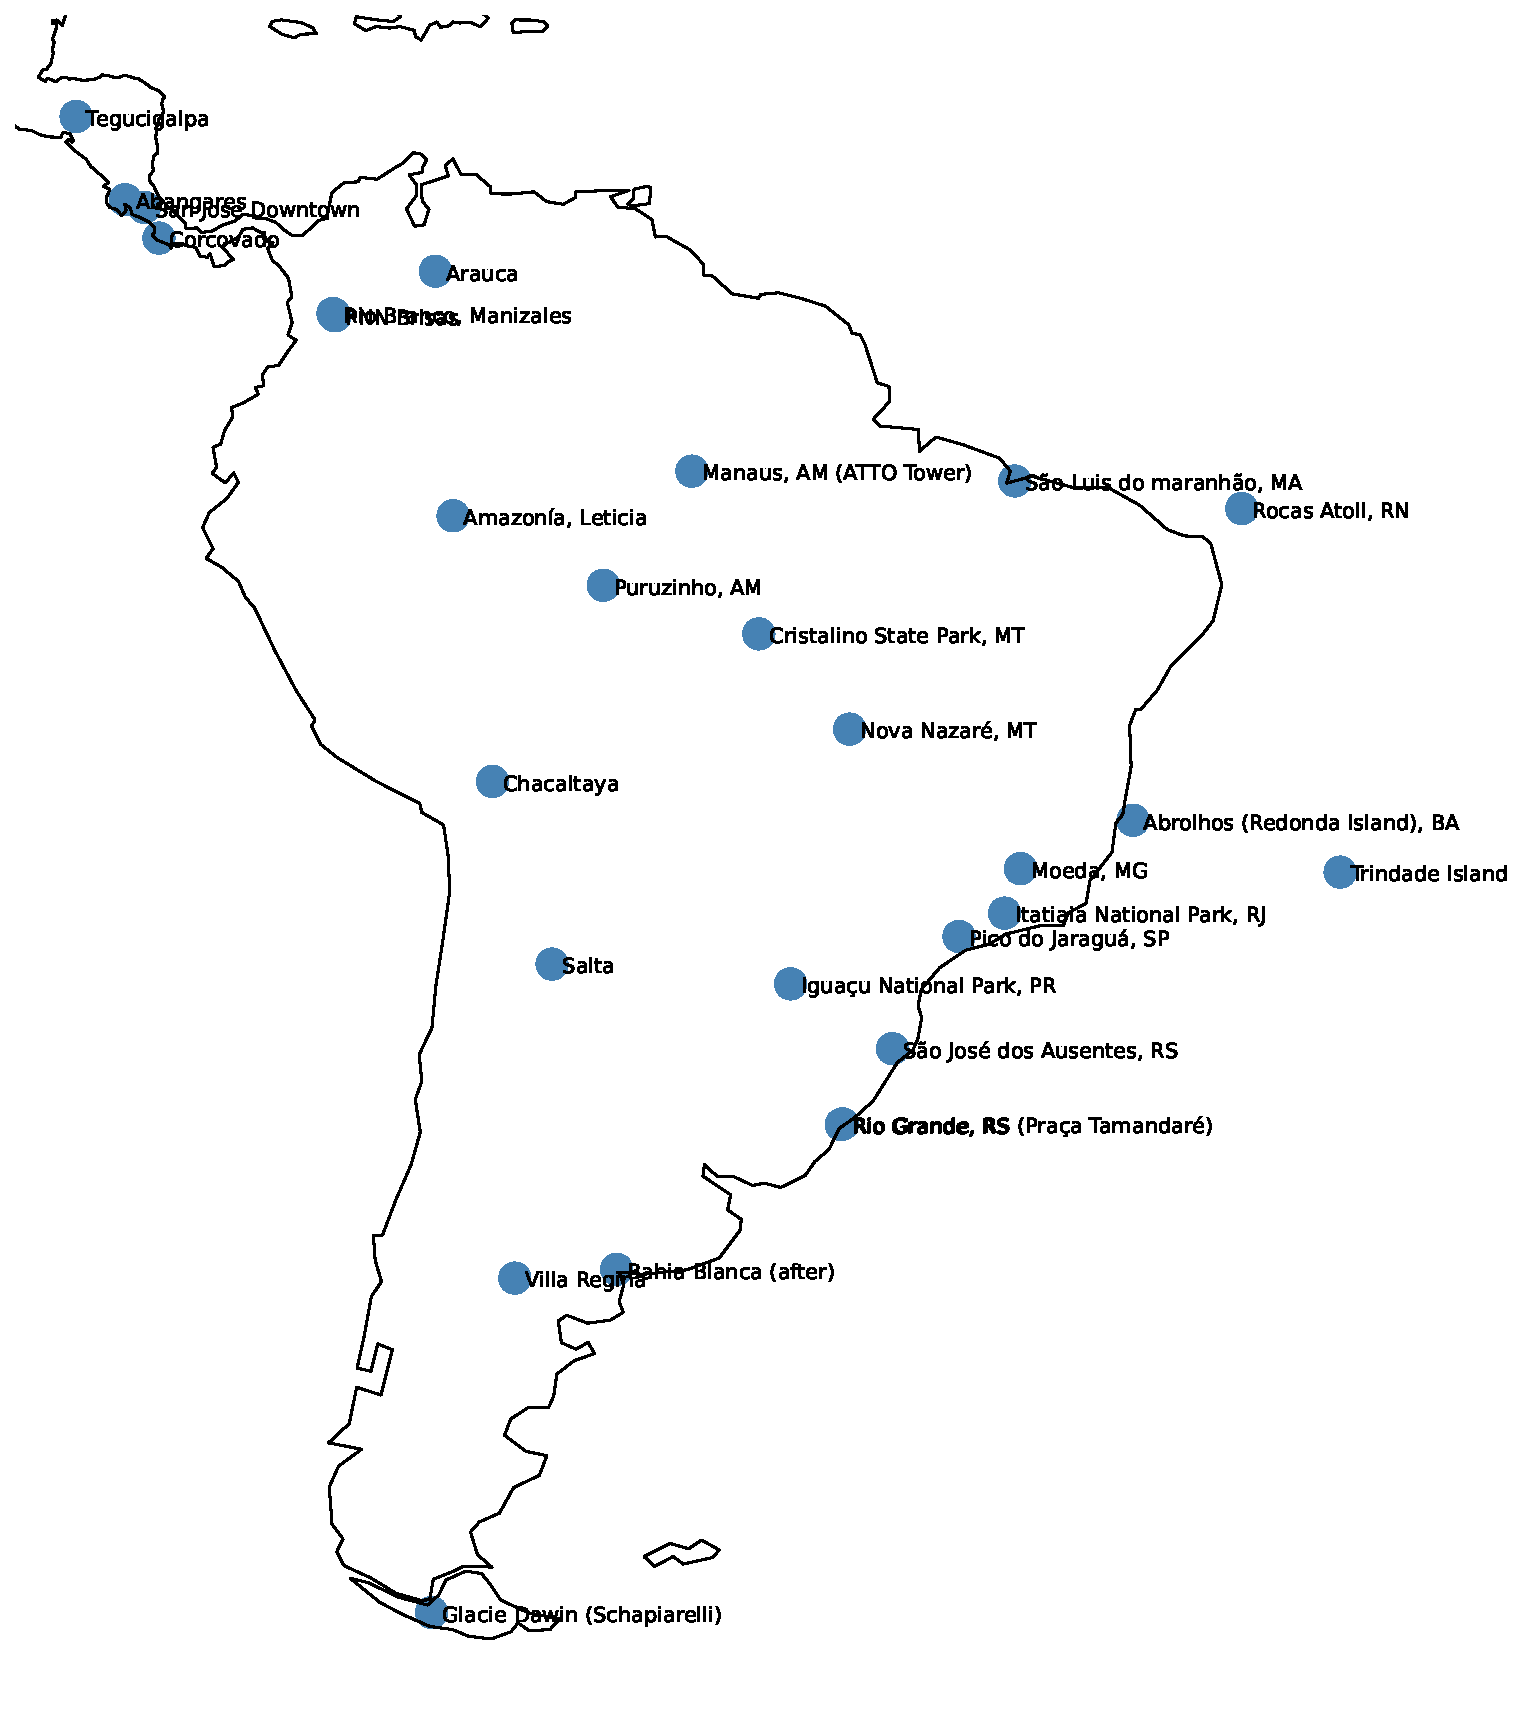
\includegraphics[width=0.8\textwidth]{templates/figures/Passive_Samplers/Latam_Passive_SamplerSites.pdf}
  \caption{Map Showing the GMOS Monitoring Network Sites and Passive Sampler Locations in South America}
  \label{fig:GMOS_PAS_stations_map}
  \centering
  
\end{figure}
\FloatBarrier



\subsection{GEOS-Chem}
\begin{flushleft}
The GEOS-Chem model (Bey et al., 2001) is used to simulate atmospheric concentrations of Hg for comparison with data constraints. GEOS-Chem is a global-scale, 3-D atmospheric chemical transport model driven by meteorological input from the Goddard Earth Observing System (GEOS) of the NASA Global Modeling and Assimilation Office. It runs at a resolution of 0.25° latitude x 0.3125° longitude horizontally, equivalent to $\approx$27 km at the equator, and 72 levels in the vertical. Numerous atmospheric chemical species have been simulated using GEOS-Chem, including Hg (Selin et al., 2008, Zhang et al., 2016, Selin et al., 2007, Holmes et al., 2010, Amos et al., 2012). Travnikov et al. (2017) also used GEOS-Chem for international model comparisons to support the Global Mercury Assessment and the Minamata Convention on Mercury.
\end{flushleft}
\begin{flushleft}

Herein we simulated the Hg concentration in the atmosphere using version 12.8.0 of GEOS-Chem at a resolution of 2.0$\times$2.5, which is equivalent to a 200 km$\times$250 km grid square at the equator. Furthermore, the GMA 2018 emissions inventory was used to represent anthropogenic emissions sources from all sectors. GEOS-Chem enables researchers to toggle different emissions sources on or off depending on the research objective, hence a Baseline simulation was created by turning on all Hg emissions sources globally. Moreover, a No-ASGM simulation was generated by turning off the ASGM source globally to figure out the contribution of ASGM to the baseline Hg concentrations in the atmosphere,which is the difference between the No-ASGM Hg concentration and the Baseline Hg concentration in the atmosphere. GEOS-Chem also allows researchers to choose the frequency of the output Hg concentration hence the global simulation was set to output daily concentration of Hg in the atmosphere while the output for the grid boxes corresponding to the locations of the GMOS was set to a hourly frequency. The GEOS-Chem outputs for all the simulations conducted were in units of parts per trillion (ppt) and were converted to nano grams per meter cube (ngm\textsuperscript{-3}) to compare them to observations.
\end{flushleft}



%%----------------------------RESULTS AND DISCUSSION---------------------------
\section{Results and Discussion}
\subsection{GMOS Observations vs GEOS-Chem}
\begin{flushleft}
Figure \ref{fig:GMOSvsGC} shows the average daily Hg concentration at the GMOS sites in red compared to the modeled average daily concentration shown by the blue line and the ASGM contribution as predicted by GEOS-Chem at the GMOS sites shown by the black line. The comparison of the GMOS observations to the GEOS-Chem model output, as seen in Figure \ref{fig:GMOSvsGC} indicated that the model generally over-estimates the observed Hg concentrations at the different GMOS sites.  With the exception of predicted concentration at the Chalcataya site, the modelled concentrations have low variability.  
\end{flushleft}


\begin{figure}[H]
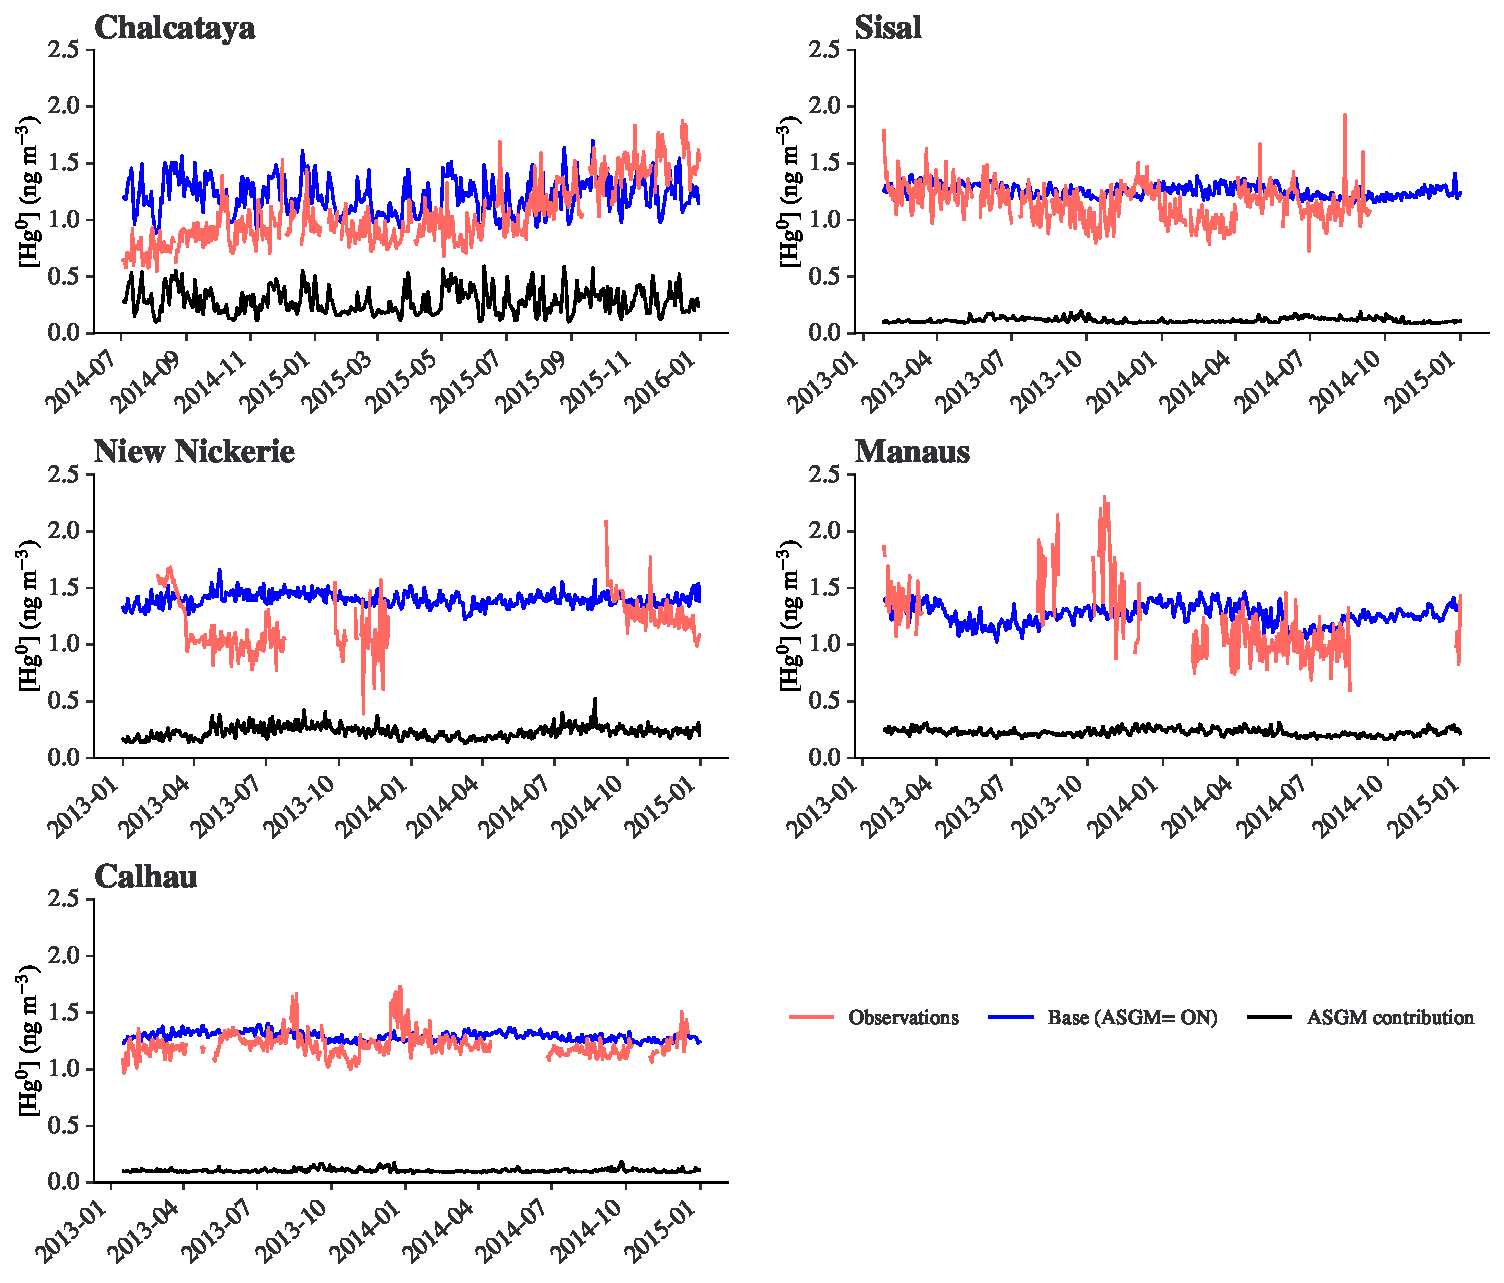
\includegraphics[width=\textwidth]{templates/figures/GMOS_Sites/GMOS_Sites.pdf}
\centering
\captionof{figure}{Plots time series plots of the observed TGM concentrations at different GMOS sites in red with the corresponding modeled concentration in blue and the associated ASGM contribution in black}
\label{fig:GMOSvsGC}
\end{figure}
\FloatBarrier

\begin{flushleft}
 Furthermore, the time series plot of the Hg concentrations at Chalcataya show a general upward trend that is not seen in the other observations and the also not predicted by the model. Table \ref{tab:ASGM_at_GMOS_annual_avs} compares the average  Hg concentration at the GMOS sites 
\end{flushleft}


\begin{table}[H]
\captionof{table}{The comparison of the model predictions of the average Hg concentration for a 1 year measurement period}
\label{tab:ASGM_at_GMOS_annual_avs}

\centering
\resizebox{\textwidth}{!}{\begin{tabular}{lcccccc}
  \hline

GMOS  &Number of& Observed Hg\textsuperscript{0} & Observation Standard & Base(ASGM=ON) Hg\textsuperscript{0} & Base(ASGM=ON) Standard  & ASGM Contribution  Hg\textsuperscript{0}   \\
Site & Records & (ng m$^{-3}$)/year             & Deviation ($\sigma$) & (ng m$^{-3}$)/year                   & Deviation ($\sigma$)      &(ng m$^{-3}$)/year\\
                        
\hline
Sisal          & 320 &1.19 & 0.14 & 1.27 & 0.05 & 0.12  \\
Calhau         & 309 &1.22 & 0.12 & 1.30 & 0.04 & 0.11  \\
Niew Nickerie  & 215 &1.11 & 0.23 & 1.41 & 0.06 & 0.25    \\
Manaus        & 100 &1.49  & 0.31 & 1.27 & 0.09 & 0.23   \\
Chalcataya     &333 &0.90 & 0.16 & 1.20 & 0.14   &0.28   \\
  \hline
\end{tabular}}

\end{table}
\begin{flushleft}
 Even though the GEOS-Chem model overestimates the mean concentration over a one year period of measurement with the exception of the Manaus site as seen in Table\ref{tab:ASGM_at_GMOS_annual_avs} the estimates for the mean concentration at Sisal and Calhau are within a 10\% margin as shown in Table \ref{tab:modelvsobs metrics}. However, the model grossly underestimates the variability in most of the GMOS sites except the Chalcataya site where the estimated standard deviation in within a 15\% margin.  
\end{flushleft}

\begin{table}[H]
\captionof{table}{Table showing the extent to which the model predicts the observations showed by the percentage difference between the model predictions and the observations }
\label{tab:modelvsobs metrics}

\centering
\resizebox{0.5\textwidth}{!}{\begin{tabular}{lcc}
  \hline

GMOS  &Percentage difference & Percentage difference  \\
Site & annual mean (\%) & standard deviation (\%)           \\
                        
\hline
Sisal          & 6.72 &-64.29  \\
Calhau         & 6.56 &-66.66   \\
Niew Nickerie  & 27.03 &-73.91    \\
Manaus        & -14.77 &-70.97    \\
Chalcataya     &33.33 &-12.5   \\
  \hline
\end{tabular}}

\end{table}
\begin{flushleft}
 The extent of the  the ASGM emissions related Hg concentration signal created by the GEOS-Chem model is prominent in only one of the GMOS sites during the measurement periods we compared to the GEOS-Chem simulation. The site that had a prominent ASGM  is mountain site at the Chalcataya (CHC) regional station, Figure \ref{fig:GMOSvsGC} (a), (World Meteorological Organization, WMO, region III-- South America; 16.35023◦ S, 68.13143◦ W),which is at an altitude of 5240 meters above sea level, about 140m below the summit of mount Chacaltaya on the eastern edge of the ``Cordillera Real,'' with a horizon open to the south and west. CHC is about 300km from the ``Madre de Dios'' watershed.
\end{flushleft}

% \begin{figure}[H]

% \begin{tabular}[H]{cc}
% \setlength{\tabcolsep}{2.5pt}

% \subfloat[Chalcataya]{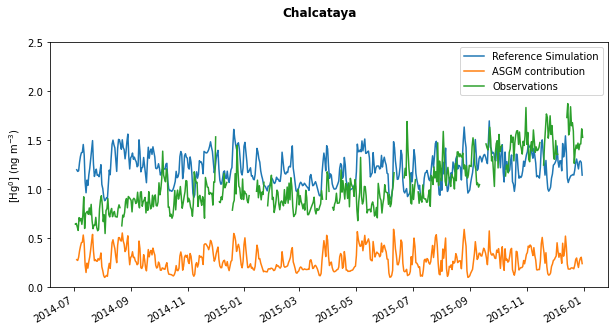
\includegraphics[width = 0.3\linewidth]{templates/figures/GMOS_Sites/chc.png}} &
% \subfloat[Sisal]{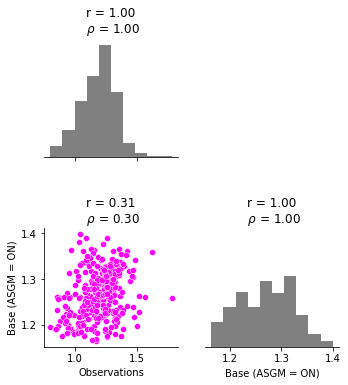
\includegraphics[width = 0.3\linewidth]{templates/figures/GMOS_Sites/sis.png}}\\

% \subfloat[Niew Nickerie]{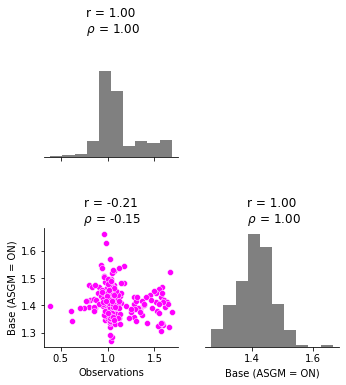
\includegraphics[width = 0.3\linewidth]{templates/figures/GMOS_Sites/NIk.png}} &
% \subfloat[Manaus]{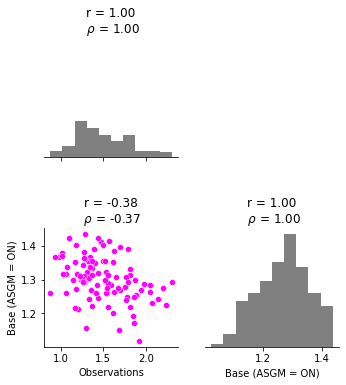
\includegraphics[width = 0.3\linewidth]{templates/figures/GMOS_Sites/man.png}}\\
% \subfloat[Calhau]{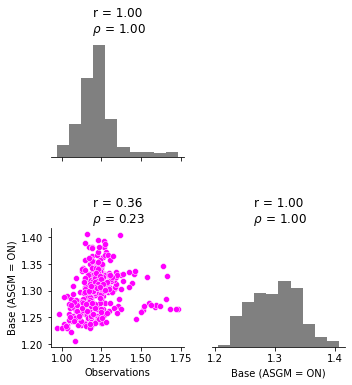
\includegraphics[width = 0.3\linewidth]{templates/figures/GMOS_Sites/cal.png}}
% \end{tabular}
% \centering
% \captionof{figure}{Sensitivity of Observations to Emission Changes in single grid box when the interquartile range (IQR) is used as the metric to compare the observations to model outputs}
% \label{fig:Histplotsiqr}
% \end{figure}
% \FloatBarrier
\subsection{Passive Sampler Observations vs GEOS-Chem}
\begin{flushleft}
 The comparison between the modelled concentration in the atmosphere and the PAS data corroborated the finding that the GEOS-Chem model overestimated the observed concentrations in the atmosphere as seen on Figure \ref{fig:06-12-22_pas_vs_model_Hg0-per-year_by-latitude_001}. Moreover the PAS observations show high variability between the south and northern locations in South America while the modeled concentrations have a low concentration. 
\end{flushleft}


\begin{figure}[H]
  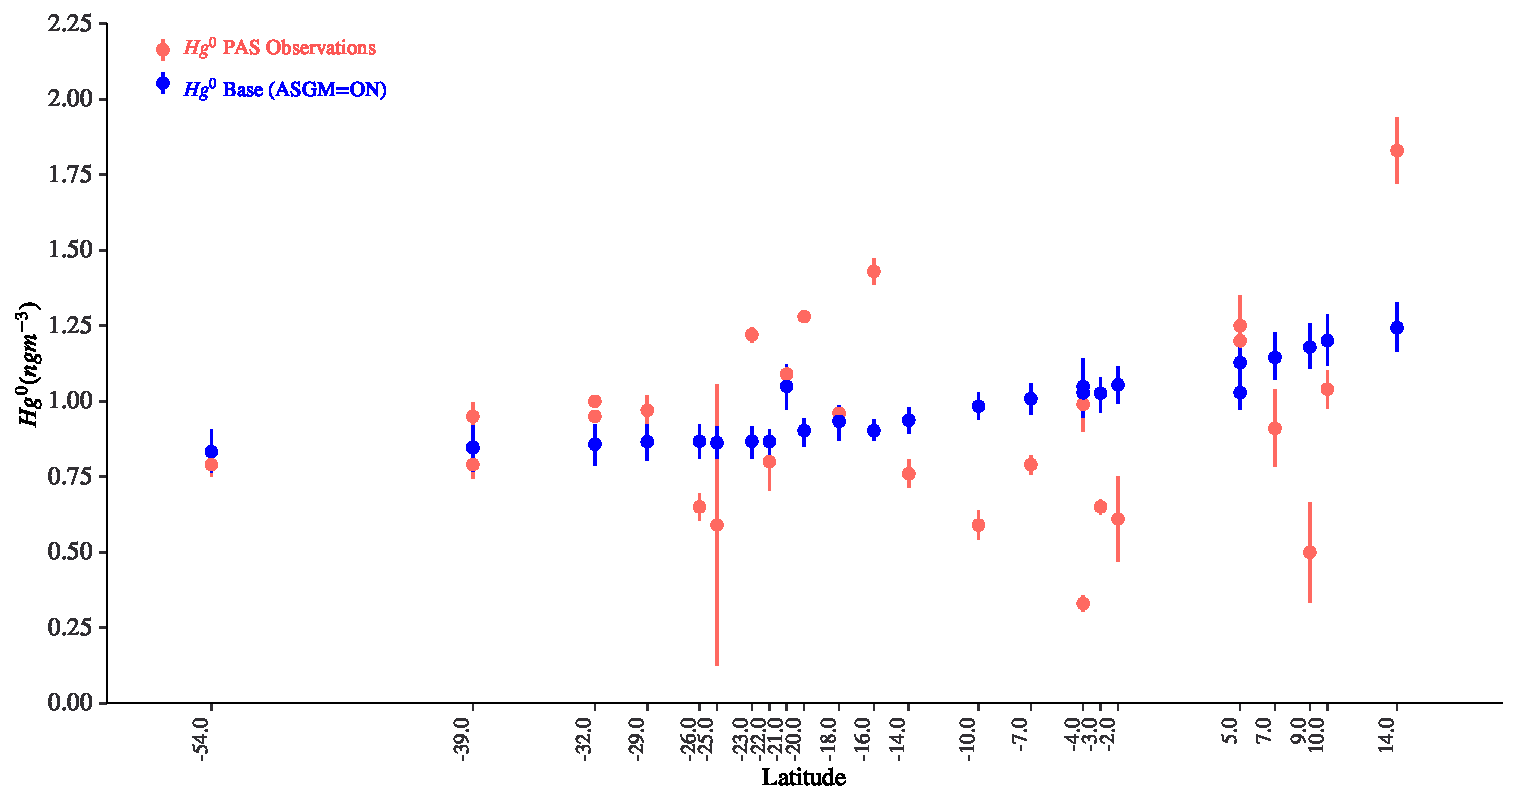
\includegraphics[width=\textwidth]{templates/figures/Passive_Samplers/06-12-22_pas_vs_model_Hg0-per-year_by-latitude_001.pdf}
  \caption{Map Showing the GMOS Monitoring Network Sites and Passive Sampler Locations in South America}
  \label{fig:06-12-22_pas_vs_model_Hg0-per-year_by-latitude_001}
  \centering
  
\end{figure}
\FloatBarrier

\begin{figure}[H]
  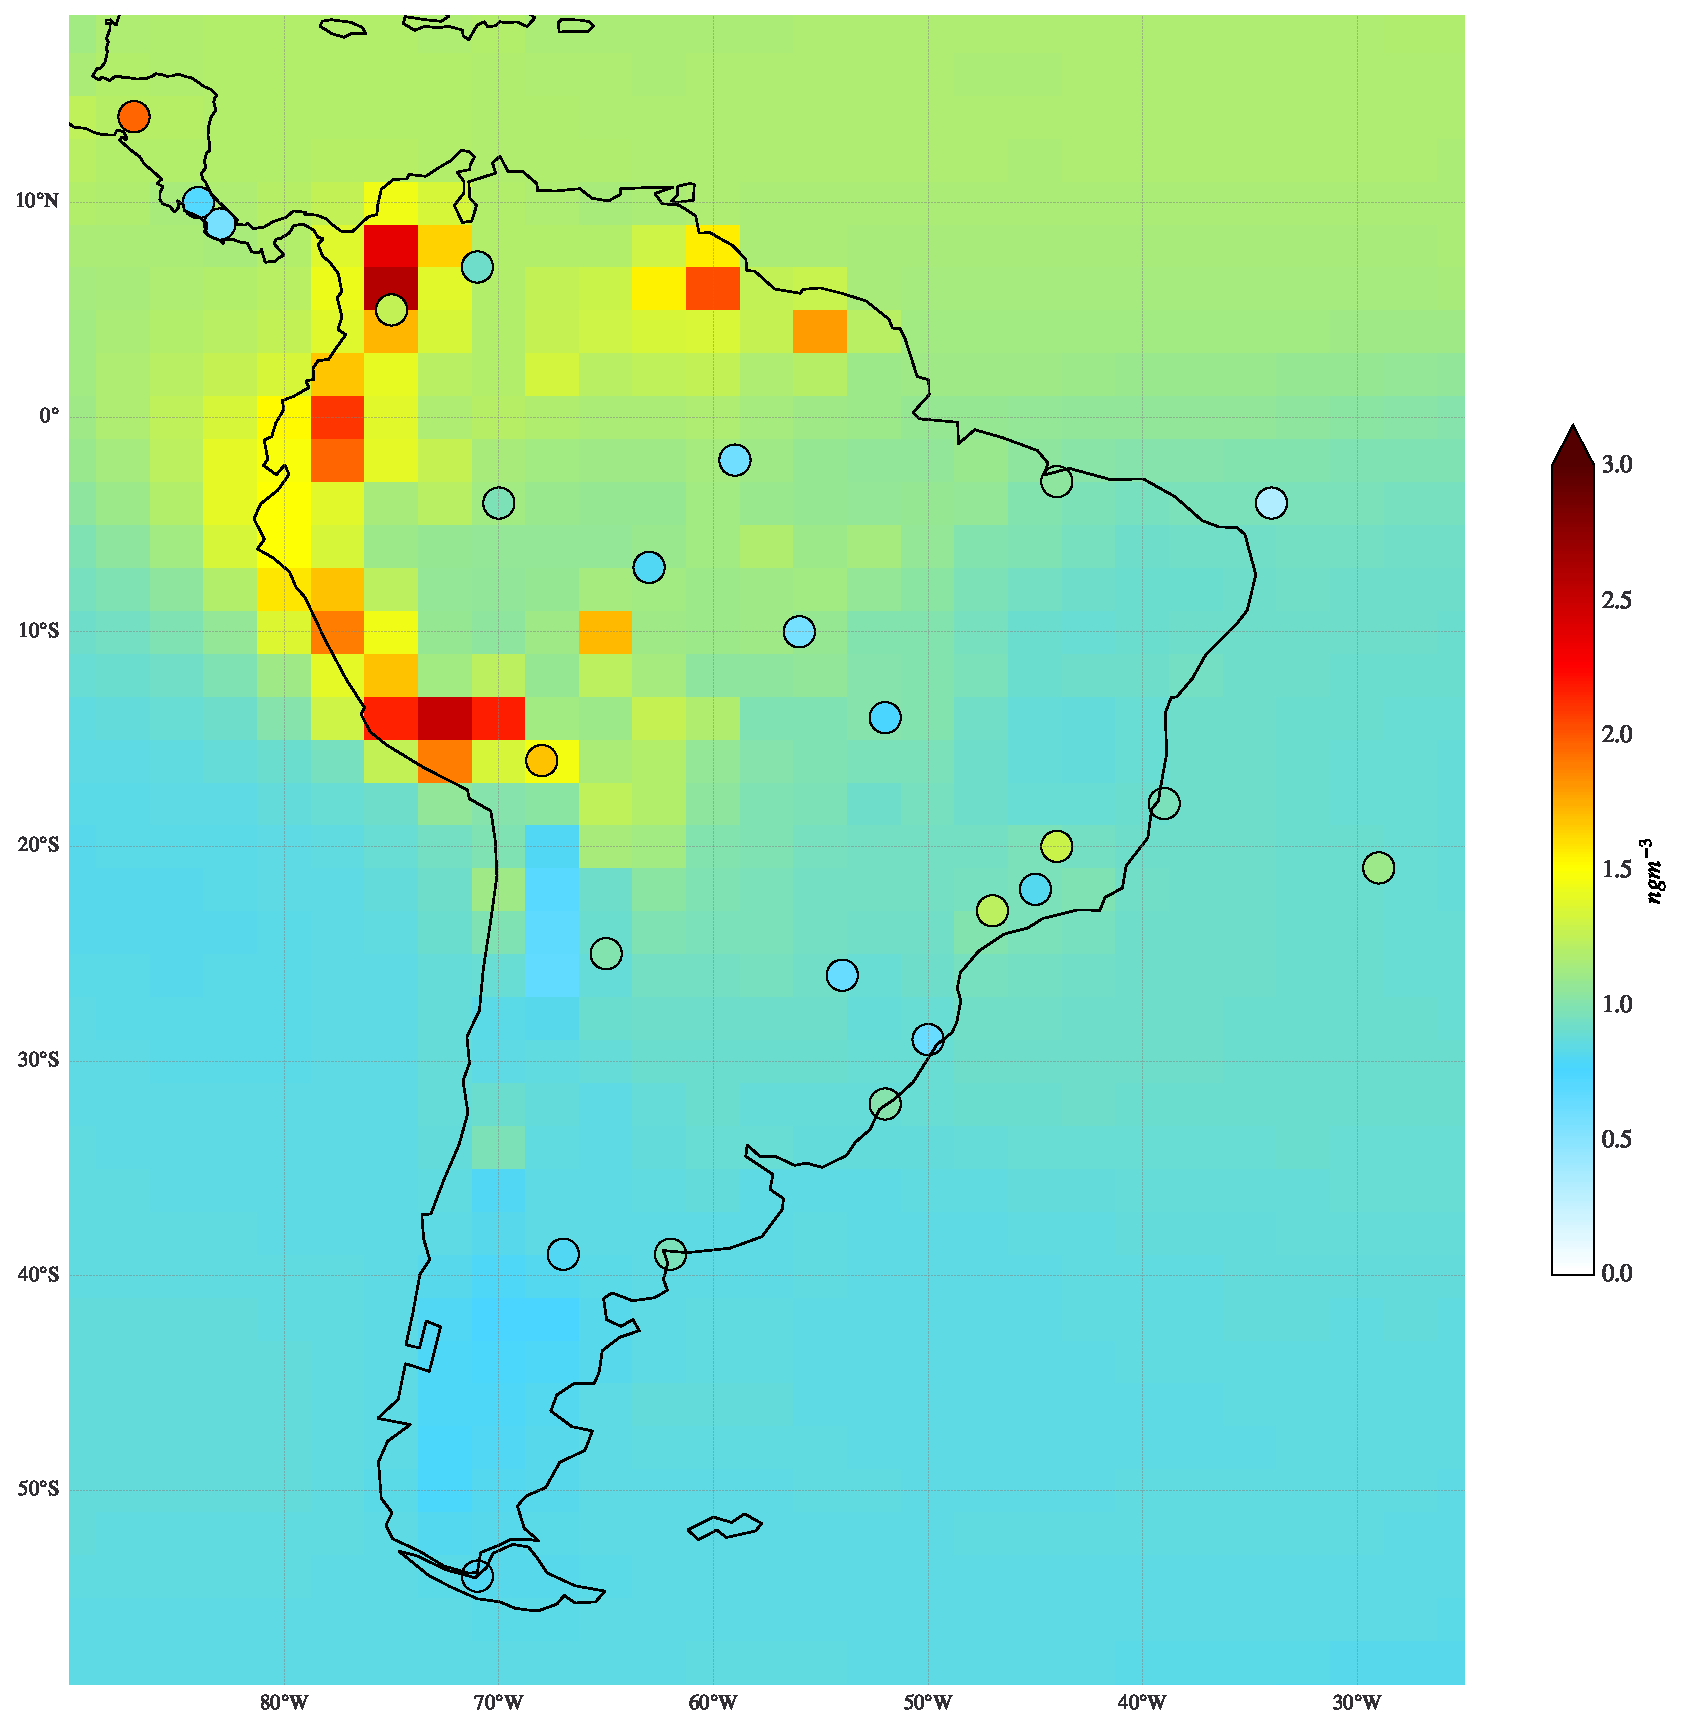
\includegraphics[width=0.7\textwidth]{templates/figures/Passive_Samplers/06-12-22_pas_vs_model_Hg0-per-year_001.pdf}
  \caption{How the predicted average annual HG concentration compares with   }
  \label{fig:06-12-22_pas_vs_model_Hg0-per-year_001}
  \centering
  
\end{figure}
\FloatBarrier

\subsection{Observed Hg Concentration at CHC}
\begin{flushleft}
The time series of the observed concentration at the CHC station between July 2014 and January 2016 is shown on Figure\ref{fig:ObsTseries}. The characteristics of the observations over this measurement period were described in Koening et all,(2020). As shown by the 120 day moving average plot on Figure\ref{fig:ObsTseries}, we found that the observed TGM concentration in the atmosphere had a visible upward trend, which Koening et all, assert was due to the El Niño-Southern Oscillation (ENSO). Consequently, they categorized the Hg concentrations in the atmosphere at the CHC site into normal conditions (NC), 2014-07 to 2015-05 and ENSO conditions  2015-06 to 2016-01. The meteorology associated with ENSO was not accounted for in the GEOS-Chem Hg model hence the GEOS-Chem simulated Hg concentration at CHC was compared to the observed Hg concentration under normal conditions.
\end{flushleft}

\begin{figure}[H]
  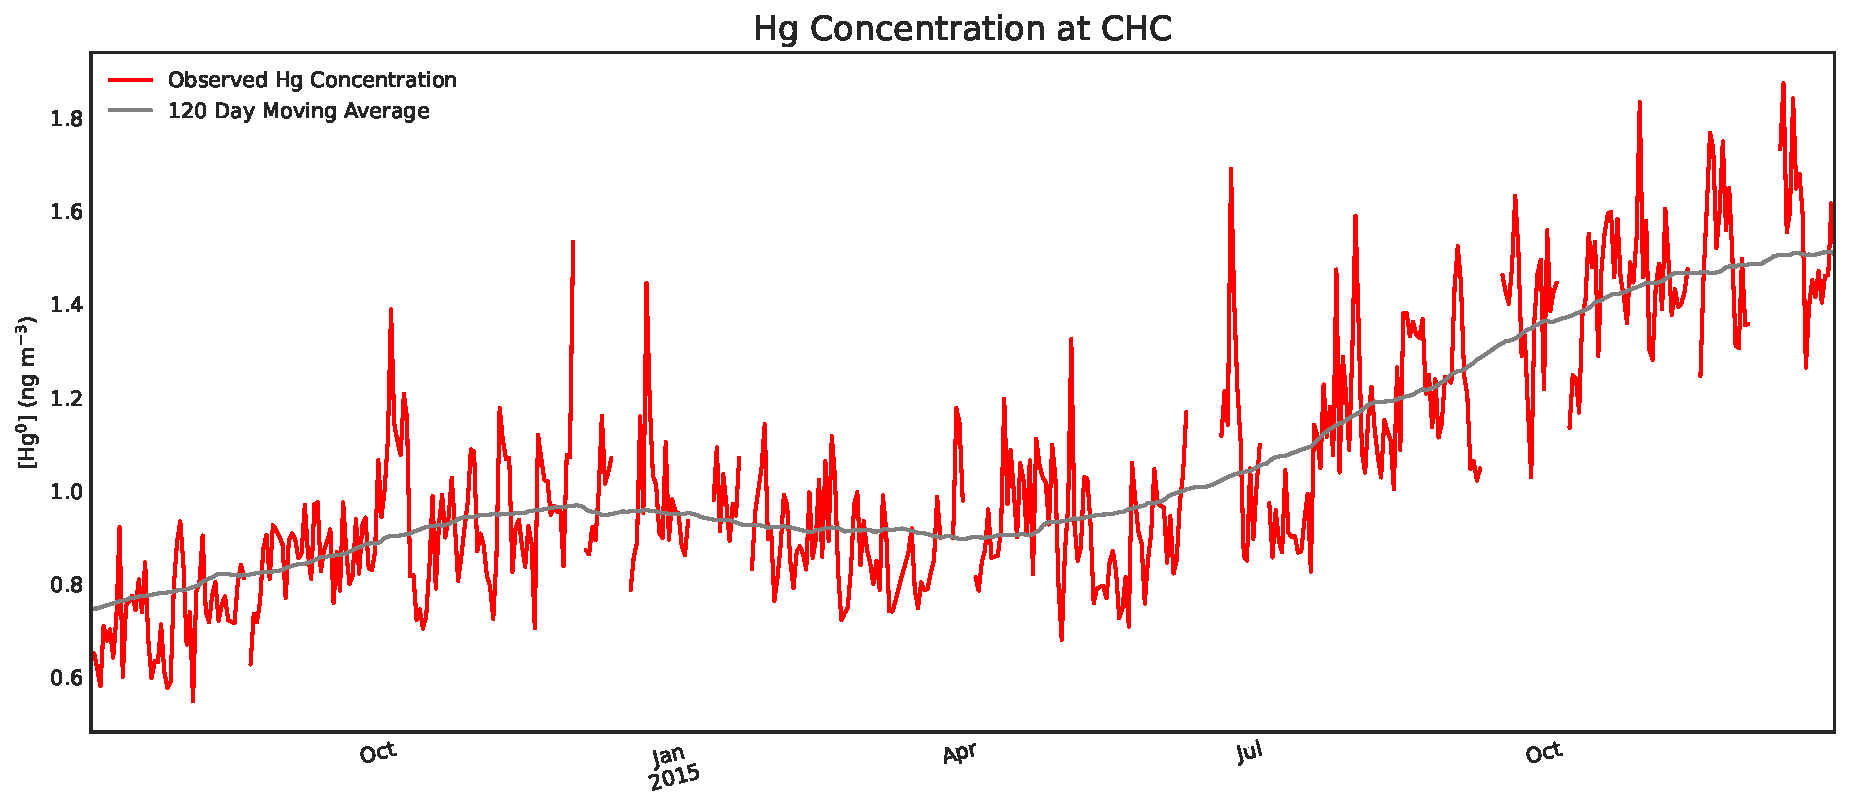
\includegraphics[width=\textwidth]{templates/figures/GMOS_Sites/ObsTimeSeries.pdf}
 
  \caption{The measured TGM concentration at CHC over the period from July 2014 to January 2016}
  \label{fig:ObsTseries}
  \centering
\end{figure}
\FloatBarrier

\begin{flushleft}
 The comparison between the observed and modelled Hg concentrations at CHC are shown on Figure \ref{fig:ModelvsObsNstats}. We found that the observed Hg concentration at CHC had an mean of 0.90 $ngm^{-3}$, which was only reproduced by the low resolution baseline GEOS-Chem simulation where global ASGM emission were turned off (LoRes Base No ASGM) shown by the green line plot. On the contrary, the low resolution baseline GEOS-Chem simulation where global ASGM emission were turned on (LoRes Base ASGM) shown by the blue line plot overestimated the mean by 29\%.
\end{flushleft}


\begin{figure}[H]
  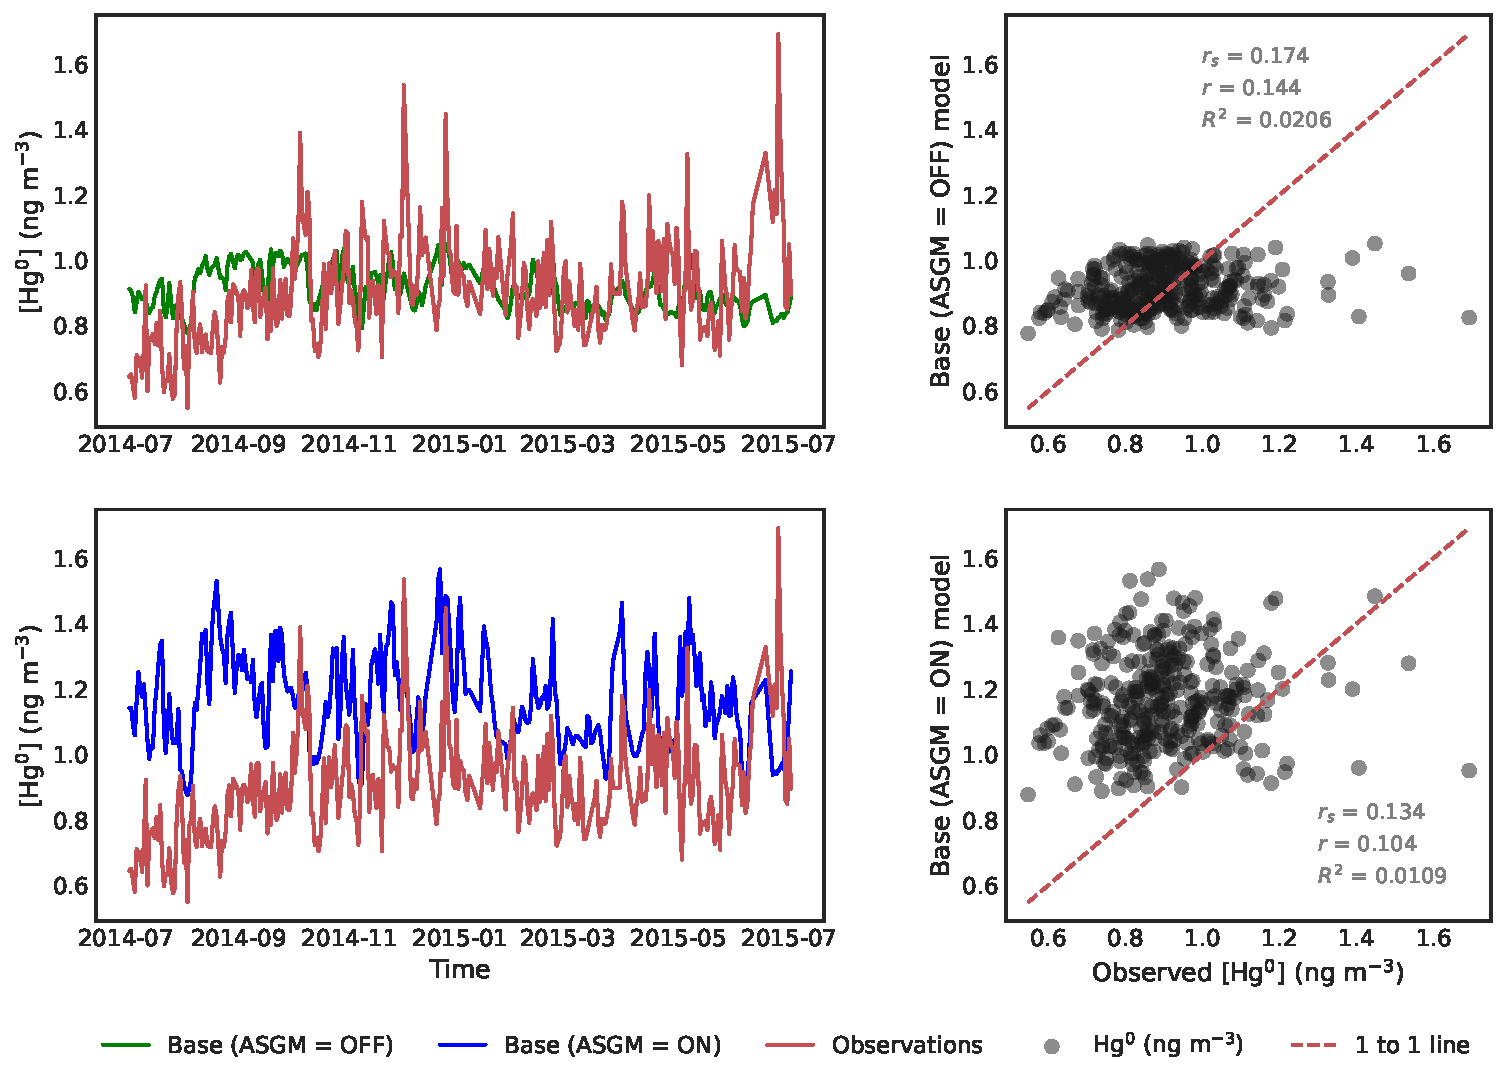
\includegraphics[width=\textwidth]{templates/figures/ModelvsObs/TimeSeriesNsactter_obsVmodel_v1.pdf}
  \centering
  \caption{Observed vs modelled (3 different simulations) Hg concentration at CHC and scatter plots of how the model compares with the observations  }
  \label{fig:ModelvsObsNstats}
\end{figure}
\FloatBarrier
\begin{flushleft}
 Similarly, the high resolution baseline GEOS-Chem simulation where global ASGM emission were turned on (HiRes Base ASGM) shown by the purple line plot overestimated the mean by 38\% as seen in Table \ref{tab:ModelvsObsStats}. Even though GEOS-Chem reproduced the mean Hg concentrations at CHC in the LoRes Base No ASGM simulation, the Spearman and Pearson correlations between the modelled and observed concentrations were very low at  1.63e-1 and 1.40e-1 respectively. Moreover, the $R^2$ between the observed and modelled concentrations in this simulation case was almost zero at 1.96e-2. Also, the LoRes No ASGM simulation did not reproduce the variability in the observed concentrations as evident in Figure \ref{fig:ModelvsObsNstats} and in Table \ref{tab:ModelvsObsStats} where we gleaned that the observations had more than twice the modelled variance. Furthermore, the observations had a higher interquartile range (IQR) than the modelled Hg concentration LoRes No ASGM case. In addition, we found that turning on ASGM emissions in GEOS-Chem led to Hg concentrations in the atmosphere that had a variance that is comparable with the variance observations as shown by the LoRes Base ASGM simulation comparison with the observations on Figure \ref{fig:ModelvsObsNstats} and Table \ref{tab:ModelvsObsStats}. However, we also discovered that turning on ASGM emissions in the model did not lead to improvements in the correlation between the modeled and observed Hg concentration in the atmosphere. 
\end{flushleft}
\setlength{\tabcolsep}{2.5pt}
\begin{table}[H]
  \begin{center}
    \caption{Characteristics of observed and modelled Hg concentration in CHC where$\mu$ is the annual average Hg concentration, $\sigma$ is the standard deviation, $iqr$ is the interquartile range, $r_s$ is the Spearman correlation, $r$ is the Pearson correlation and $R^2$ is the coeeficient of determination}
    \label{tab:ModelvsObsStats}
    \begin{tabular}{lcccccc}
       %<-- added & and content for each column
      
                          & $\mu$                 & $\sigma$            & $iqr$               & & & \\
                          &  (ng m$^{-3}$)/year)  & (ng m$^{-3}$)/year) & (ng m$^{-3}$)/year) & & & \\
     \cmidrule{2-4}
     Observations         & 0.90             & 0.16            & 0.18        &  & & \\
     \textbf{Simulations} &                  &                  &               &\textbf{$r_s$} &\textbf{$r$} &\textbf{$R^2$}\\ %
      \hline
      Base (ASGM=OFF)     & 0.91             & 0.06            & 0.11         & 0.17         & 0.144      & 0.0196\\ 
      Base (ASGM=ON)      & 1.16            & 0.14            & 0.20        & 0.124         & 0.101       & 0.0102\\ % <--
    \end{tabular}
  \end{center}
\end{table}
\FloatBarrier

\begin{flushleft}
The relationship between the mean and variance in the observed and modeled Hg concentration in the atmosphere at CHC was further explored as shown on Figure \ref{fig:Histplots} which shows the extent to which that the GEOS-Chem model recreates the mean and IQR of the observations. Even though the LoRes Base ASGM simulation better recreated the IQR of the Hg concentration in the atmosphere, the mean Hg concentration in this simulation was almost two standard deviations away from the mean of the observations. Consequently, we determined that the mean was not a good metric to investigate the relationship between the Hg concentration in the atmosphere and ASGM emissions as modelled by GEOS-Chem. 
\end{flushleft}



\begin{figure}[H]

\begin{tabular}[H]{cc}

\subfloat[]{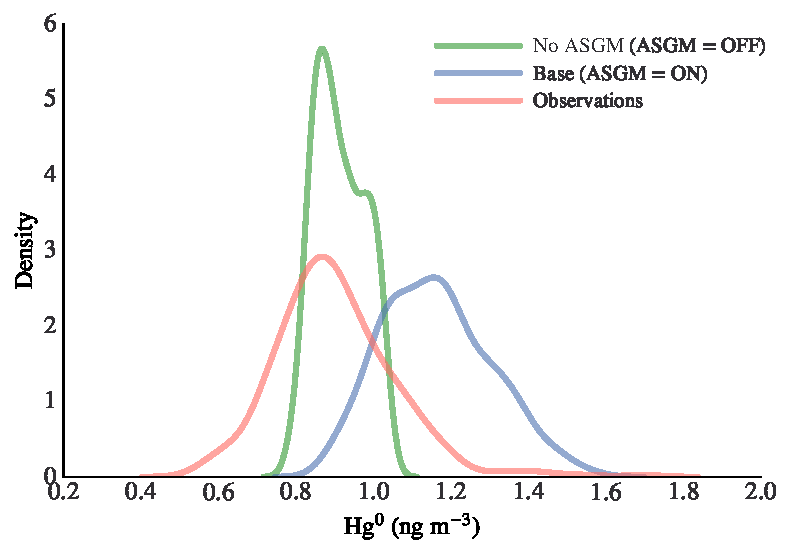
\includegraphics[width = 0.5\linewidth]{templates/figures/ModelvsObs/06-12-22_models_vs_observations_density-plot.pdf}} &
\subfloat[]{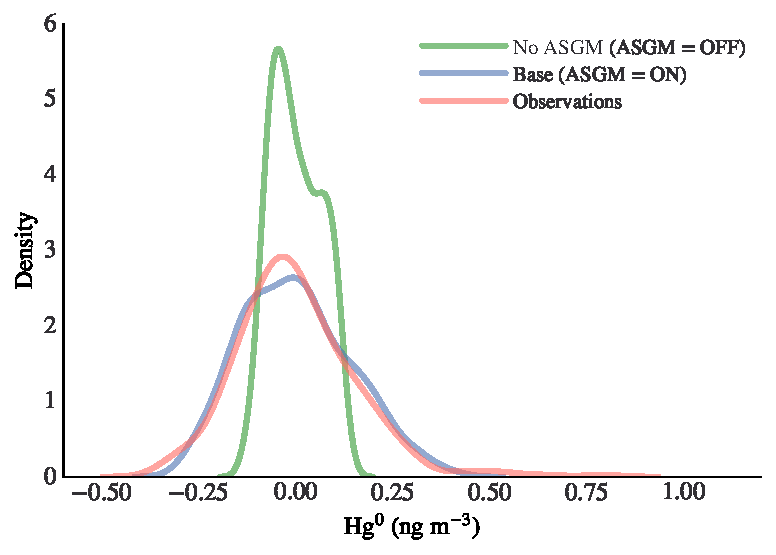
\includegraphics[width = 0.5\linewidth]{templates/figures/ModelvsObs/06-12-22_models_vs_observations_density-plot_std.pdf}}
\end{tabular}
\centering
\captionof{figure}{Plots Showing Data and Modeling  Results from GMOS Monitoring Network Sites in South America}
\label{fig:Histplots}
\end{figure}
\FloatBarrier

\begin{flushleft}
Instead, the IQR and $95^{th}$ percentile range were found to be metrics that were informative about the effect of ASGM on the simulated Hg concentration site at distant high altitude measuring station site. The failure of GEOS-Chem to reproduce the observed mean Hg concentration at a high altitude measuring site may be attributed to poor parameterizations in the model such as the influence of dry deposition. The flaws in the GEOS-Chem Hg dry deposition scheme in version 12.8.1 of GEOS-Chem used in this analysis were discussed in detail and improved in Feinberg et.al (2022). Furthermore, we hypothesized that poor spatial distribution of emissions in the 2015 Hg ASGM emissions inventory which are an input to the GEOS-Chem may have also contributed to the model observation mismatches. 
% The discrepancy in the distribution of emissions is evidence in the comparison of a national inventory of Peruvian ASGM emissions as produced by the Artisanal Gold Council and the emission estimates from the GMA2018 in Table \ref{tab:gamVagc}.
\end{flushleft}

% \begin{table}[H]
% \caption{}
%     \label{tab:gamVagc}
% \begin{tabular}{lcc}

% \textbf{Region}        & \textbf{GMA 2018}    & \textbf{Artisanal Gold Counsel}                          \\
% \hline
% Madre de Dios & & \\

% Apurimac      & &\\

% Arequipa      & & \\

% North Puno    & & \\

% South Puno    & & \\
% \hline
% \end{tabular}
% \centering
% \end{table}




\section{Conclusion}

